\section{Interazioni neutrino-fermione}
Questo è un argomento di ricerca ancora aperto costruendo fasci di neutrini studiando soprattutto l'oscillazione. Noi li studiamo qua perché è diverso dal decadimento di una particella per vedere le interazioni deboli. Inoltre il neutrino è risultato anche estremamente importante come sonda per studiare i nucleoni e poi tutto questo formalismo che sviluppiamo viene leggermente modificato per capire come studiare le correnti deboli neutre che non abbiamo ancora visto. L'interazione corrente-corrente di Fermi può essere utilizzata per calcolare le sezioni d'urto di interazioni neutrino fermione mediate da corrente carica (CC). Può essere utilizzata anche per descrivere interazioni di antineutrini e può essere utilizzata per interazioni di neutrini di tutte le famiglie. 
\begin{figure}[h!]
	\centering
	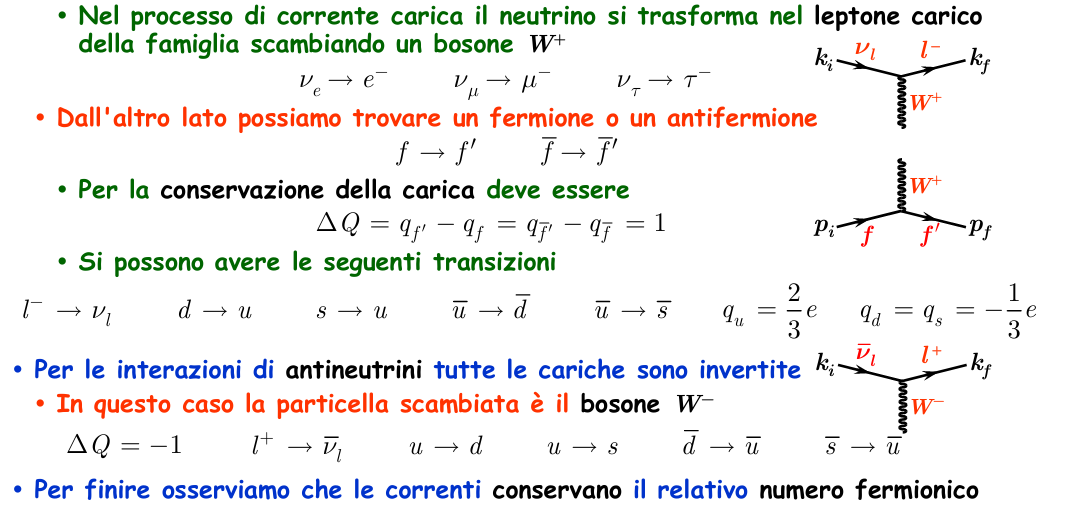
\includegraphics[width=0.9\textwidth]{Lezioni/Lezione 18/lez.png}
	\label{fig:ledz}
\end{figure}
Troveremo la stessa formula per tutte le famiglie anche se in realtà le famiglie differiscono per la massa ma spesso queste masse le approssimeremo a zero (fenomeni ad alta energia). Le formule per le particelle sono diverse da quelle per le antiparticelle sia per i neutrini-antineutrini che per i fermioni-antifermioni. Per fissare le idee studiamo:
\begin{itemize}
	\item La sezione d'urto neutrino elettronico - elettrone
	\item La seizone d'urto antineutrino elettronico - elettrone
\end{itemize}
Questi due processi sono mediati da correnti sia cariche che neutre
\begin{figure}[h!]
	\centering
	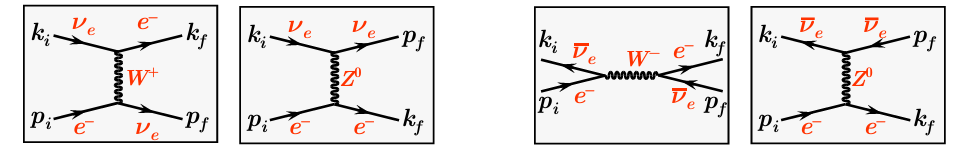
\includegraphics[width=0.9\textwidth]{Lezioni/Lezione 18/reaz.png}
	\label{fig:reaz}
\end{figure}
Per il momento trascureremo la corrente neutra anche se sono indistinguibili i due processi per quanto riguarda i risultati finali e quindi si scrivono le due ampiezze e si fa il modulo quadro ma trascureremo per il momento questo discorso. La reazione $\bar{\nu}_\mu e^-\to\mu^-\nu_e$ può essere mediata solo tramite CC mentre osserviamo che la reazione $\bar{\nu}_\mu e^-\to\bar{\nu}_\mu e^-$ può essere mediata solo da corrente neutra.
\begin{figure}[h!]
	\centering
	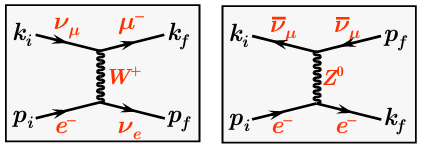
\includegraphics[width=0.5\textwidth]{Lezioni/Lezione 18/reaz1.png}
	\label{fig:reaz1}
\end{figure}
\section{Lo scattering $\nu_e e^-\to\nu_e e^-$}
Iniziamo con il calcolo della sezione d'urto per lo scattering di un neutrino da parte di un elettrone
$$
\nu_e + e^- \to \nu_e + e^-
$$
Il diagramma di Feynman al primo ordine associato a questa reazione e la corrispondente ampiezza di Fermi sono
\begin{figure}[h!]
	\centering
	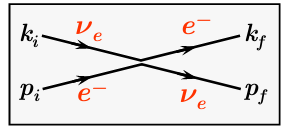
\includegraphics[width=0.3\textwidth]{Lezioni/Lezione 18/reaz2.png}
	\label{fig:reaz2}
\end{figure}
Il quadrato dell'elemento di matrice è
$$
\mathfrak{M} = \frac{G}{\sqrt{2}} \bar{u}_{k_f} \gamma^\mu (1 - \gamma^5) u_{k_i} \bar{u}_{p_f} \gamma_\mu (1 - \gamma^5) u_{p_i}
$$
$$
\overline{|\mathfrak{M}|^2} = \frac{G^2}{2} M^{\mu\nu} N_{\mu\nu}
$$
I due tensori $M^{\mu\nu}$ e $N^{\mu\nu}$ sono facilmente derivabili dal diagramma utilizzando le regole per i diagrammi
$$
M^{\mu\nu} = Tr\left[ (\slashed{k}_f + m_e) \gamma^\mu (1 - \gamma^5) (\not{k}_i + m_\nu) (1 + \gamma^5) \gamma^\nu \right]
$$
$$
N^{\mu\nu} = \frac{1}{2} Tr\left[ (\slashed{p}_f + m_\nu) \gamma^\mu (1 - \gamma^5) (\slashed{p}_i + m_e) (1 + \gamma^5) \gamma^\nu \right]
$$
Nel primo tensore non è fatta la media sulle polarizzazioni iniziali (manca il fattore $\frac{1}{2}$) perché il neutrino ha solo lo stato left-handed. Il calcolo delle tracce è lasciato come esercizio. Il risultato per i due tensori è $(m_\nu=0)$
$$
M^{\mu\nu} = 8 \left[ k_i^\mu k_f^\nu - g^{\mu\nu} k_i \cdot k_f + k_f^\mu k_i^\nu - i \varepsilon^{\lambda\mu\sigma\nu} k_{i\lambda} k_{f\sigma} \right]
$$
$$
N^{\mu\nu} = 4 \left( p_i^\mu p_f^\nu - g^{\mu\nu} p_i \cdot p_f + p_f^\mu p_i^\nu - i \varepsilon^{\lambda\mu\sigma\nu} p_{i\lambda} p_{f\sigma} \right)
$$
Il prodotto dei due tensori si calcola facilmente (un po' lungo...) infatti occorre la proprietà del tensore di Levi-Civita
$$
-\varepsilon^{\mu\nu\lambda\sigma} \varepsilon_{\mu\nu\alpha\beta} = 2 \left( \delta_\alpha^\lambda \delta_\beta^\sigma - \delta_\beta^\lambda \delta_\alpha^\sigma \right)
$$
Il risultato è
$$
\overline{|\mathfrak{M}|^2} = \frac{G^2}{2} 128 (k_i \cdot p_i)(k_f \cdot p_f)
$$
Calcoliamo i prodotti: dalla conservazione del $4-$momento
$$
k_i + p_i = k_f + p_f
$$
$$
s = (k_i + p_i)^2 = (k_f + p_f)^2 \qquad s = 2k_i \cdot p_i + m_e^2 = m_e^2 + 2k_f \cdot p_f
$$
Trascuriamo $m_e$
$$
k_i \cdot p_i = k_f \cdot p_f = \frac{s}{2}
$$
Inserendo nell'elemento di matrice si ottiene
$$
\overline{|\mathfrak{M}|^2} = \frac{G^2}{2} 128 \frac{s^2}{4} = 16 G^2 s^2
$$
La sezione d'urto è
$$
d\sigma = \frac{\overline{|\mathfrak{M}|^2}}{4\sqrt{(k_i \cdot p_i)^2 - (m_e m_\nu)^2}} d\Phi_2
$$
Ricordiamo il fattore di flusso $F$ e lo spazio delle fasi $d\Phi_2$
$$
F = 4\sqrt{(p_1 \cdot p_2)^2 - (m_1 m_2)^2} = 4|\mathbf{q}_i|W_i \qquad d\Phi_2 = \frac{1}{(4\pi)^2} \frac{|\mathbf{q}_f|}{W_f} d\Omega
$$
Inoltre
$$
|\mathbf{q}_i| = |\mathbf{q}_f| = \frac{\sqrt{s}}{2} \qquad W_i = W_f = \sqrt{s}
$$
Otteniamo pertanto
$$
d\Phi_2 = \frac{1}{2} \frac{d\Omega}{(4\pi)^2} \qquad F = 4\sqrt{(p_1 \cdot p_2)^2 - (m_1 m_2)^2} = 2s
$$
Per l'elemento di matrice il risultato del calcolo era
$$
\overline{|\mathfrak{M}|^2} = \frac{G^2}{2} 128 \frac{s^2}{4} = 16 G^2 s^2
$$
Introducendo nella formula per la sezione d'urto
$$
d\sigma = 16 G^2 s^2 \frac{1}{2s} \frac{1}{2} \frac{d\Omega}{(4\pi)^2}
$$
Pertanto, nel centro di mass, la sezione d'urto è isotropa
$$
\frac{d\sigma}{d\Omega} = \frac{G^2 s}{4\pi^2}
$$
La sezione d'urto totale è
$$
\sigma = \int \frac{G^2 s}{4\pi^2} d\Omega = \frac{G^2 s}{\pi}
$$
\section{Lo scattering $\bar{\nu}_e e^-\to\bar{\nu}_e e^-$}
Calcoliamo adesso il quadrato dell'ampiezza della reazione
$$
\overline{\nu}_e + e^- \to \overline{\nu}_e + e^-
$$
Il diagramma di Feynman al primo ordine (solo CC) associato a questa reazione e la corrispondente ampiezza di Fermi sono
\begin{figure}[h!]
	\centering
	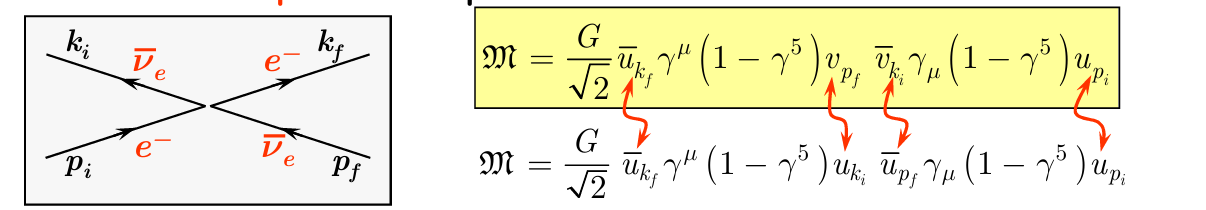
\includegraphics[width=0.7\textwidth]{Lezioni/Lezione 18/reaz3.png}
	\label{fig:reaz3}
\end{figure}
Le correnti sono relative a particelle o tutte nello stato iniziale o tutte nello stato finale. Nella reazione neutrino-elettrone le correnti univano particelle fra gli stati iniziali e finali. Confrontiamo la corrispondente ampiezza della reazione $\nu_e e^-\to\nu_e e^-$. Gli spinori $u_{kf}$ e $u_{pi}$ compaiono allo stesso modo e quindi contribuiranno allo stesso modo.
\begin{itemize}
	\item Lo spinore $u_{ki}$ è diventato $v_{pf}$ ma dato che $m_\nu=0$ basta sostituire $k_i$ con $p_f$.
	\item Lo spinore $u_{pf}$ è diventato $v_{ki}$ ma dato che $m_\nu=0$ basta sostituire $p_f$ con $k_i$.
\end{itemize}
Sostituendo (la tecnica che viene usata è detta crossing)
$$
\overline{|\mathfrak{M}|^2} = \frac{G^2}{2} 128 (k_i \cdot p_i)(k_f \cdot p_f) \quad \implies \quad \overline{|\mathfrak{M}|^2} = \frac{G^2}{2} 128 (p_f \cdot p_i)(k_f \cdot k_i)
$$
Questa reazione è uguale al fatto che porto una particella che passo dallo stato iniziale a quello finale facendola diventare antiparticella e viceversa. Studiamo adesso la cinematica della reazione. Consideriamo la conservazione del $4-$momento
$$
k_i + p_i = k_f + p_f
$$
Possiamo ricavare una espressione utile per la variabile di Mandelstam t
$$
k_i - k_f = p_f - p_i \qquad t = (k_i - k_f)^2 = (p_f - p_i)^2
$$
Trascurando ancora una volta le masse delle particelle
$$
t = -2k_i \cdot k_f = -2p_i \cdot p_f
$$
Consideriamo adesso il sistema del centro di massa dato che lo scattering è elastico
$$
\mathbf{p}_i = -\mathbf{k}_i \quad \mathbf{p}_f = -\mathbf{k}_f \quad |\mathbf{k}_i| = |\mathbf{k}_f| \equiv |\mathbf{q}| \quad E = |\mathbf{q}| \quad |\mathbf{q}| = \frac{\sqrt{s}}{2}
$$
Calcoliamo t (sempre trascurando le masse)
$$
t = -2k_i \cdot k_f = -2E_1E_3 + 2(\mathbf{k}_i \cdot \mathbf{k}_f) = -2\mathbf{q}^2 + 2\mathbf{q}^2 \cos\theta = -2\mathbf{q}^2(1 - \cos\theta)
$$
$$
t = -\frac{s}{2}(1 - \cos\theta)
$$
Inseriamo i risultati nell'elemento di matrice
$$
\overline{|\mathfrak{M}|^2} = 4G^2s^2(1 - \cos\theta)^2
$$
Quindi a differenza della reazione precedente questa ci da un elemento di matrice che non è costante in funzione dell'angolo di diffusione. Prima avevamo una sezione d'urto isotropa in questo caso invece non lo è. Lo spazio delle fasi e il flusso sono identici al caso precedente e inserendo nella formula per la sezione d'urto otteniamo
$$
\frac{d\sigma}{d\Omega} = \frac{G^2s}{(4\pi)^2}(1 - \cos\theta)^2
$$
Per la sezione d'urto totale integriamo su tutto l'angolo solido trovando un risultato diverso (più piccolo con quel fattore $3$)
$$
\sigma = \int_{-1}^{1} \frac{G^2s}{(4\pi)^2}(1 - \cos\theta)^2 2\pi d\cos\theta \quad \sigma = \frac{G^2s}{3\pi}
$$
Riepiloghiamo i risultati ottenuti
$$
\nu_e + e^- \to \nu_e + e^- \quad \frac{d\sigma}{d\Omega} = \frac{G^2s}{4\pi^2} \quad \sigma = \frac{G^2s}{\pi}
$$
$$
\bar{\nu}_e + e^- \to \bar{\nu}_e + e^- \quad \frac{d\sigma}{d\Omega} = \frac{G^2s}{(4\pi)^2}(1 - \cos\theta)^2 \quad \sigma = \frac{G^2s}{3\pi}
$$
Si può comprendere la differenza tra i due risultati facendo riferimento alla conservazione del momento angolare e alla violazione di parità
\begin{figure}[h!]
	\centering
	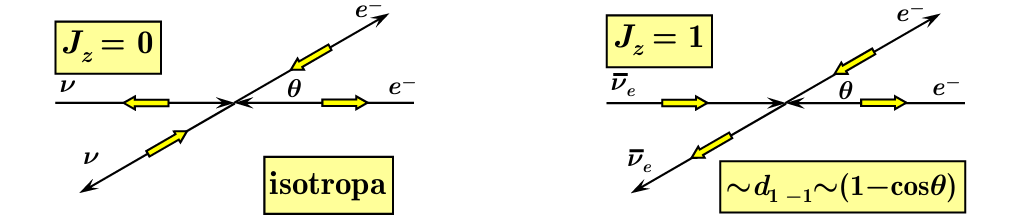
\includegraphics[width=0.8\textwidth]{Lezioni/Lezione 18/reaz4.png}
	\label{fig:reaz4}
\end{figure}
\section{Interazione neutrino quark (CC)}
\begin{figure}[h!]
	\centering
	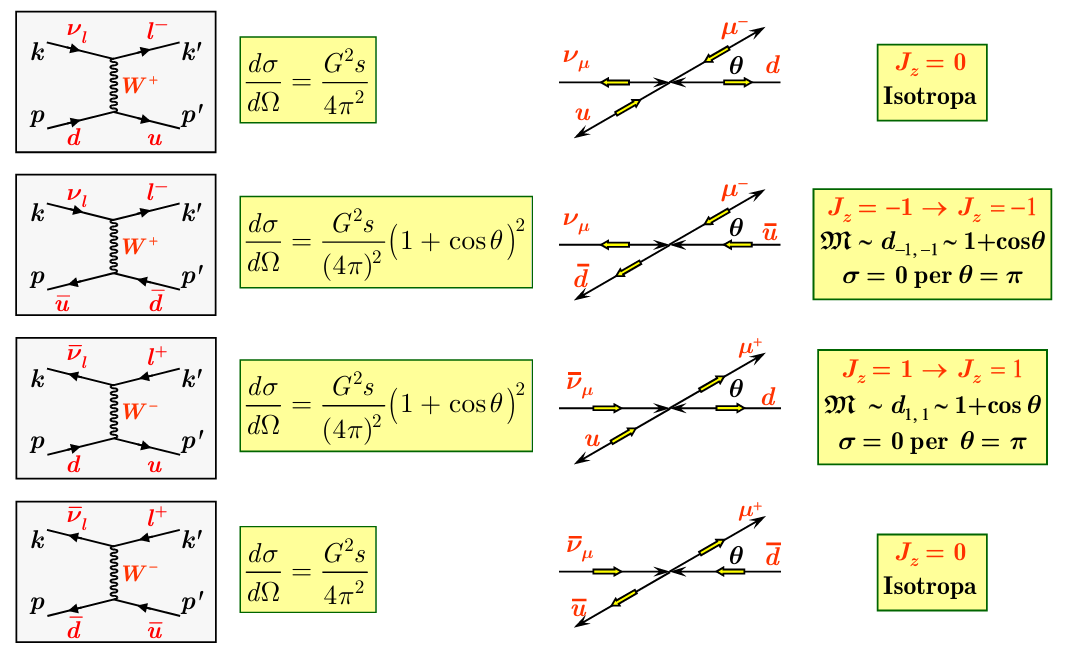
\includegraphics[width=0.8\textwidth]{Lezioni/Lezione 18/reaz5.png}
	\label{fig:reaz5}
\end{figure}
Nella prima reazione vedo un neutrino che interagisce con un quark. Se andiamo a vedere abbiamo particelle e quindi sono tutte LH ed ho momento $J_z=0$ quindi isotropo! Se andiamo a fare interazione con un anti-fermione e andiamo a vedere quello che succede nella configurazione del momento angolare quindi abbiamo che $\mathfrak{M}$ è proporzionale a $d_{-1,-1}$ che è proporzionale a $(1+\cos(\theta))$. E così via con le quattro interazione con neutrino e leptone o antileptone.
\section{La reazione $\nu_\mu e^-\to\mu^-\nu_e$}
Includiamo l'effetto della massa del leptone carico che è importante per la reazione in quanto il muone è più pesante dell'elettrone
$$
\nu_\mu e^-\to\mu^-\nu_e
$$
La struttura dell'elemento di matrice è identica ma l'unica differenza è la massa del muone. Nei casi precedenti, il calcolo del quadrato dell'elemento di matrice era stato fatto senza approssimazioni fino al risultato.
$$
\overline{|\mathfrak{M}|^2} = 64G^2 (k_i \cdot p_i)(k_f \cdot p_f)
$$
Che è esatto e non contiene l'approssimazione di massa nolla. Adesso calcoliamo i due prodotti scalari. Per il primo, relativo ai momenti nello stato iniziale, non ci sono modifiche (si può trascurare $m_e$). 
$$
k_i \cdot p_i = \frac{s}{2}
$$
Per il secondo prodotto abbiamo
$$
s = (k_f + p_f)^2 = m_\mu^2 + 2k_f \cdot p_f \qquad k_f \cdot p_f = \frac{s - m_\mu^2}{2} = \frac{s}{2} \left( 1 - \frac{m_\mu^2}{s} \right)
$$
Inserendo dell'elemento di matrice
$$
\overline{|\mathfrak{M}|^2} = 16G^2 s^2 \left( 1 - \frac{m_\mu^2}{s} \right)
$$
Per spazio delle fasi e flusso non si può usare il calcolo precedente ma con cura. Quando trascuriamo le masse le reazioni sono processi di scattering elastico. le masse delle particelle nello stato iniziale sono uguali alle masse nello stato finale. La quantità di moto (3d) nel centro di massa dello stato iniziale è uguale alla quantità di moto nel centro di massa dellos tato finale. Nel caso della reazione
$$
\nu_\mu + e^- \to \mu^- + \nu_e
$$
Le masse delle particelle nello stato iniziale e finale sono diverse. Di conseguenza le quantità di moto $q_i$ e $q_f$ sono differenti. Le quantità di moto nel flusso e nello spazio delle fasi sono differenti. Ricordiamo il risultato per il fattore di flusso
$$
\sqrt{(p_1 \cdot p_2)^2 - (m_1m_2)^2} = \frac{s}{2}
$$
Questo risultato è ancora valido perché la cinematica dello stato iniziale non è cambiata. Ricordiamo il risultato per lo spazio delle fasi occorre esprimere $q_f$ in termini di invarianti e occorre tenere conto dell'effetto soglia (infatti devo avere abbastanza energia per produrre quella massa nello stato finale che non avevo nello stato finale. Non solo bisogna avere quella massa ma anche conservare la quantità di moto quindi l'energia del neutrino deve essere molto maggiore rispetto a quella che ci aspettiamo)
$$
d\Phi_2 = \frac{1}{(4\pi)^2} \frac{|\mathbf{q}_f|}{\sqrt{s}} d\Omega
$$
Saltando i conti cinematici trovo che la formula dello spazio delle fasi nel nostro caso
$$
d\Phi_2 = \frac{1}{(4\pi)^2} \frac{|\mathbf{q}_f|}{\sqrt{s}} d\Omega \qquad |\mathbf{q}_f| = \frac{s - m_\mu^2}{2\sqrt{s}}
$$
Otteniamo
$$
d\Phi_2 = \frac{1}{(4\pi)^2} \frac{s - m_\mu^2}{2s} d\Omega \qquad d\Phi_2 = \frac{1}{(4\pi)^2} \frac{1}{2} \left( 1 - \frac{m_\mu^2}{s} \right) d\Omega
$$
Inserendo questi risultati nella formula per la sezione d'urto
$$
d\sigma = \frac{\overline{|\mathfrak{M}|^2}}{4\sqrt{(k \cdot p)^2 - (m_e m_{\nu_\mu})^2}} d\Phi_2
$$
$$
\overline{|\mathfrak{M}|^2} = 16G^2 s^2 \left( 1 - \frac{m_\mu^2}{s} \right) \qquad \sqrt{(p_1 \cdot p_2)^2 - (m_1 m_2)^2} = \frac{s}{2}
$$
Otteniamo
$$
\frac{d\sigma}{d\Omega} = \frac{G^2 s}{4\pi^2} \left( 1 - \frac{m_\mu^2}{s} \right)^2 \qquad E_\nu \ge \frac{m_\mu^2 - m_e^2}{2m_e} = 10.79 \text{ GeV}
$$
Questa è l'energia minima! Per produrre un muone con un'energia di circa $105\,\unit{MeV}$ il neutrino deve avere un'energia così tanto maggiore!
\section{Difficoltà dell'Interazione di Fermi}
Le sezioni d'urto fin qui calcolate divergono al crescere dell'energia. Osserviamo inoltre che i calcoli fin qui fatti sono approssimati al primo ordine della teoria perturbativa. Sorge quindi spontaneo chiedersi se è possibile fare calcoli di ordine superiore ad esempio includendo diagrammi a loop. Ma purtroppo diagrammi di questo tipo divergono. Il tipo di divergenza è grave e non si riesce a reinterpretare come invece avviene per l'elettrodinamica con la rinormalizzazione. La teoria di Fermi infatti non è rinormalizzabile. Si è tentato di rendere la teoria più simile all'elettrodinamica introducendo il bosone vettoriale intermedio (IVB). Le correnti dell'interazione di Fermi sono vettoriali. La particella scambiata deve essere un $4-$vettore, spin $1$. L'interazione debole è a corto range (al limite di contatto) e quindi la particella scambiata deve avere una massa non nulla. Dobbiamo trovare il propagatore di una particella vettoriale di massa non nulla. Approfondiamo lo studio dei propagatori.
\section{Il propagatore del bosone $W^{\pm}$}
La stessa derivazione può essere fatta per il propagatore di bosoni vettoriali con massa diversa da zero. Una prima differenza sta nella relazione fra energia e quantità di moto
$$
q_0 = |\mathbf{q}| = \sqrt{\mathbf{q}^2} \to q_0 = \sqrt{\mathbf{q}^2 + m^2}
$$
Una seconda differenza risiede nel valore delle somme di polarizzazioni
$$
\sum_{\lambda=1}^3 \varepsilon_\lambda^\mu(k)\varepsilon_\lambda^\nu(k) = -\left(g^{\mu\nu} - \frac{1}{m^2}k^\mu k^\nu\right)
$$
Tenendo conto di questa differenza il propagatore per una particella vettoriale di massa $M_W$ è
$$
D^{\mu\nu}(q) = \frac{1}{q^2 - M_W^2 + i\epsilon} \left(-g^{\mu\nu} + \frac{q^\mu q^\nu}{M_W^2}\right)
$$
Infatti avendo massa a differenza del fotone ha uno stato di polarizzazione in più.
Calcoliamo l'ampiezza di transizione per un processo che abbiamo descritto con l'interazione corrente-corrente utilizzando il propagatore
\begin{figure}[h!]
	\centering
	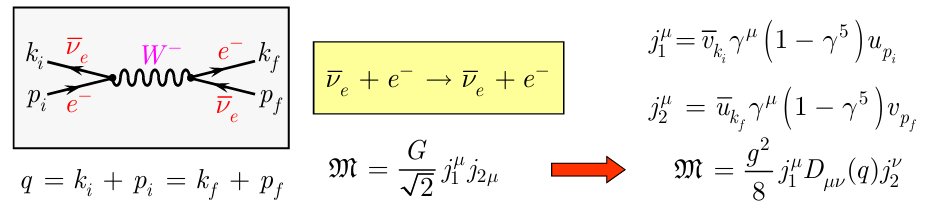
\includegraphics[width=0.9\textwidth]{Lezioni/Lezione 18/reaz6.png}
	\label{fig:reaz6}
\end{figure}
Utilizziamo la formula esplicita del propagatore
$$
j_1^\mu = \overline{v}_{k_i} \gamma^\mu (1 - \gamma^5) u_{p_i} \qquad j_2^\mu = \overline{u}_{k_f} \gamma^\mu (1 - \gamma^5) v_{p_f}
$$
$$
\mathfrak{M} = \frac{1}{8} \frac{g^2}{q^2 - M_W^2 + i\varepsilon} j_1^\mu \left( -g_{\mu\nu} + \frac{q_\mu q_\nu}{M_W^2} \right) j_2^\nu
$$
Consideriamo prima il pezzo del propagatore che contiene i termini $q_\mu q_\nu$ ricordando che $q=k_i+p_i=k_f+p_f$ e calcoliamo il contributo della prima corrente
$$
q_\mu j_1^\mu = \overline{v}_{k_i} \gamma^\mu (k_i + p_i)_\mu (1 - \gamma^5) u_{p_i} = \overline{v}_{k_i} (\slashed{k}_i + \slashed{p}_i) (1 - \gamma^5) u_{p_i}
$$
$$
= m_e \overline{v}_{k_i} (1 + \gamma^5) u_{p_i} - m_\nu \overline{v}_{k_i} (1 - \gamma^5) u_{p_i}
$$
$$
\overline{v}_{k_i} \slashed{k}_i = -m_\nu \overline{v}_{k_i}\qquad \not{p}_i u_{p_i} = m_e u_{p_i}
$$
Un risultato analogo per la seconda corrente 
$$
q_\nu j_2^\nu = m_e \overline{v}_{k_f} (1 - \gamma^5) u_{p_f} - m_\nu \overline{v}_{k_f} (1 + \gamma^5) u_{p_f}
$$
In definitiva i contributi sono proporzionale a termini ($a,b=e,\nu$) che sono contributi trascurabili. Osservazioni: la corrente debole non è conservata e sarebbe conservata per masse nulle.
$$
\frac{m_a m_b}{M_W^2}
$$
\section{Il modello Bosone Vettoriale Intermedio (IVB)}
Consideriamo il termine proporzionale a $g_{\mu\nu}$. La costante $g$ introdotta gioca il ruolo della carica $e$
$$
\mathfrak{M} = -\frac{g^2}{8} \frac{j_1^\mu g_{\mu\nu} j_2^\nu}{q^2 - M_W^2 + i\varepsilon}
$$
Consideriamo il limite di momento trasferito trascurabile
$$
q^2 \ll M_W^2
$$
In questo limite l'ampiezza diventa
$$
\mathfrak{M} = \frac{g^2}{8M_W^2} j_1^\mu j_{2\mu} \quad \text{da confrontare con }\quad \mathfrak{M} = \frac{G}{\sqrt{2}} j_1^\mu j_{2\mu}
$$
Si arriva pertanto alla identificazione
$$
G = \frac{\sqrt{2}}{8} \frac{g^2}{q^2 - M_W^2} \quad \Rightarrow \quad G = \sqrt{2} \frac{g^2}{8M_W^2}
$$
Concludiamo che al primo ordine dello sviluppo perturbativo i risultati trovati con l'interazione corrente-corrente possono essere generalizzati al modello IVB semplicemente sostituendo $G$ con l'espressione contenente il propagatore. In particolare la sezione d'urto
$$
\bar{\nu}_e + e^- \to \bar{\nu}_e + e^-
$$
Non è più divergente nel limite di alta energia e la divergenza per $s=M_W^2$ è apparente (abbiamo trascurato $\Gamma_W$)
$$
\sigma = \frac{G^2s}{3\pi} \quad \Rightarrow \quad \sigma = \frac{g^4s}{3 \cdot 32\pi} \frac{1}{(s - M_W^2)^2}
$$
Purtroppo, nonostante l'apparente successo, il modello IVB non è ancora una soluzione soddisfacente. Esistono diagrammi di ordine superiore con più propagatori. La particelle $W^{\pm}$ introdotta può partecipare a reazioni in cui è reale e non virtuale. Questi diagrammi divergono in modo non rinormalizzabile.